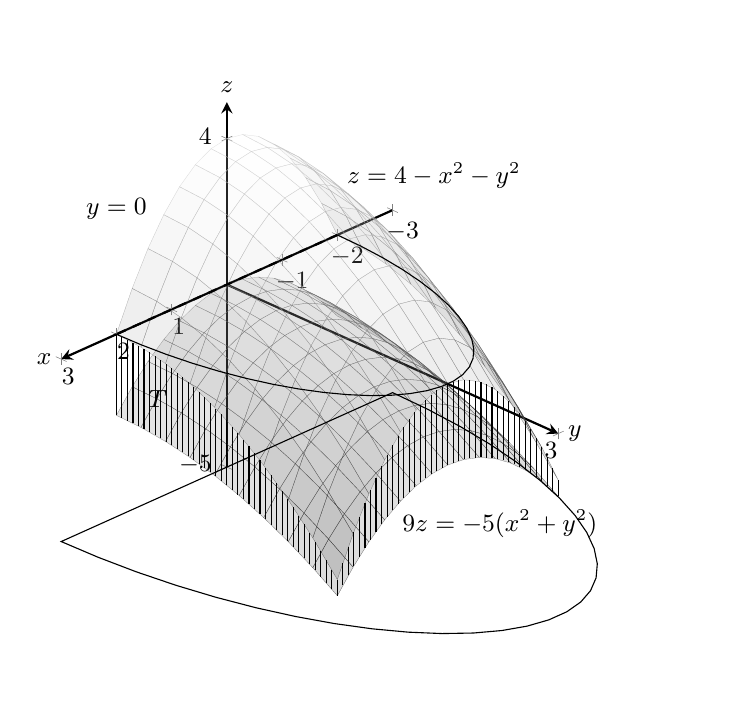
\begin{tikzpicture}
\begin{axis}[
    axis lines=middle,
    axis line style={thick, black},
    view={135}{30},
    xlabel=$x$, xlabel style={left},
    ylabel=$y$, ylabel style={right},
    zlabel=$z$, zlabel style={above},
    xmin=-3, xmax=3,
    ymin=0, ymax=3,
    zmin=-5, zmax=5,
    xtick={-3,...,3},
    ytick={3},
    ztick={-5,4},
    width=10cm,
    height=10cm,
    clip=false,
    colormap/blackwhite,
    grid=major,
    grid style={dashed, black!30},
    axis background/.style={fill=white},
    tick label style={font=\small},
    label style={font=\small}
]

\addplot3[
    surf,
    domain=-2:2,
    domain y=0:2,
    samples=15,
    samples y=10,
    opacity=0.6,
    fill opacity=0.15,
    line width=0.1pt
] {-5/9*(x^2 + y^2)};

\node[anchor=north west, font=\small] at (axis cs:1,2,-2.5) {$9z=-5(x^2+y^2)$};

\addplot3[
    surf,
    domain=-2:2,
    domain y=0:2,
    samples=15,
    samples y=10,
    opacity=0.6,
    fill opacity=0.15,
    line width=0.1pt
] {4 - x^2 - y^2};

\node[anchor=south west, font=\small] at (axis cs:-2,0,1) {$z=4-x^2-y^2$};

\addplot3[
    black,
    dashed,
    line width=0.8pt
] coordinates {
    (-2,0,0) (2,0,0)
};

\node[anchor=north, font=\small] at (axis cs:2,0,4) {$y=0$};

\pgfplotsinvokeforeach{0,0.05,...,2} {
    \draw[black] (2,#1,{-20/9-5/9 * #1^2}) -- (2,#1,{- #1^2});
}

\pgfplotsinvokeforeach{-2,-1.9,...,0} {
    \draw[black] (#1,2,{-20/9+5/9 * #1^2}) -- (#1,2,{+ #1^2});
}

\pgfplotsinvokeforeach{0,0.1,...,2} {
    \draw[black] (#1,2,{-20/9-5/9 * #1^2}) -- (#1,2,{- #1^2});
}

\addplot3[
    domain=0:180,
    samples=30,
    black,
    dashed,
    line width=0.4pt
] ({2*cos(x)}, {2*sin(x)}, {4 - 4});

\addplot3[
    domain=0:180,
    samples=30,
    dashed,
] ({3*cos(x)}, {3*sin(x)}, -5);

\node[anchor=west, font=\small, color=black] at (axis cs:2,0.2,-1.5) {$T$};

\end{axis}
\end{tikzpicture}